\section{Three Prediction Problems}
\label{sec:schema}

To understand hypotheses H1-H3, consider three corresponding prediction problems in Figure~\ref{fig:three-prediction-problems}(a)-(c): action interpolation (P1), action transfer (P2) and shape transfer (P3). Consider how each might be tackled using either: (i) rigid body simulator employing classical mechanics or (ii) statistical machine learning. Assume object and environment shape to be known.

\subsection{Action Interpolation (P1)} Suppose some pushes of an object were made (Figure~\ref{fig:three-prediction-problems} (a) top row). In some cases the object tipped, in some it slid. Now a new push direction is tried (bottom row, left column). The task is to predict the new object motion. To do this, rigid body mechanics requires parameters such as the object mass and frictional coefficients. These may be estimated from the available data. Thus, even for a classical mechanics approach, the problem involves learning. Alternatively, generalisation across actions is feasible using semi- or non-parametric machine learning. This is because the experiences span the test case: there aren't any exactly similar actions, but there are many with similar features. Hence, this problem involves {\em action interpolation}.

\subsection{Action Transfer (P2)} Figure~\ref{fig:three-prediction-problems} (b) depicts a harder problem since the test action (bottom row) now sits outside the range of training actions. Hence, this problem is known as {\em action transfer}. Turning the object around, since it is not symmetric, means that the effects of actions are quite different than before. For example, pushing the top of the L-shaped object will no longer induce it to tip over. This is because the horizontal flap cannot pass through the table: it provides a {\em kinematic constraint} on the motion of the object. This makes action transfer problems challenging for tabula rasa machine learning. Such problems should, however, be no more challenging for rigid body simulation than problem P1, since once an object's parameters are estimated, the rigid body simulator can produce predictions for any action.

\subsection{Shape Transfer (P3)} Finally, Figure~\ref{fig:three-prediction-problems} (c) requires generalising predictions about action effects to novel shapes. The training data consists of pushes of two objects of different shape. The test action is a push of an object of novel shape. This is a challenge for learning because small changes in object shape can lead to large changes in behaviour. The problem is also challenging for an approach that uses a tuned rigid body simulator, since estimation of mass and frictional coefficients for the test object must be based on the estimates made from the training data, and will thus be sensitive to estimation errors.

Problems P2 and P3 arise from quite different kinds of variation, but in fact are quite similar. Both require learning of the possible motion types at contacts. By learning models of contact behaviour, rather than whole object motion, both problems can be solved in essentially the same way.

\subsection{The case for modular prediction learning}
\begin{figure}[t]
\centerline{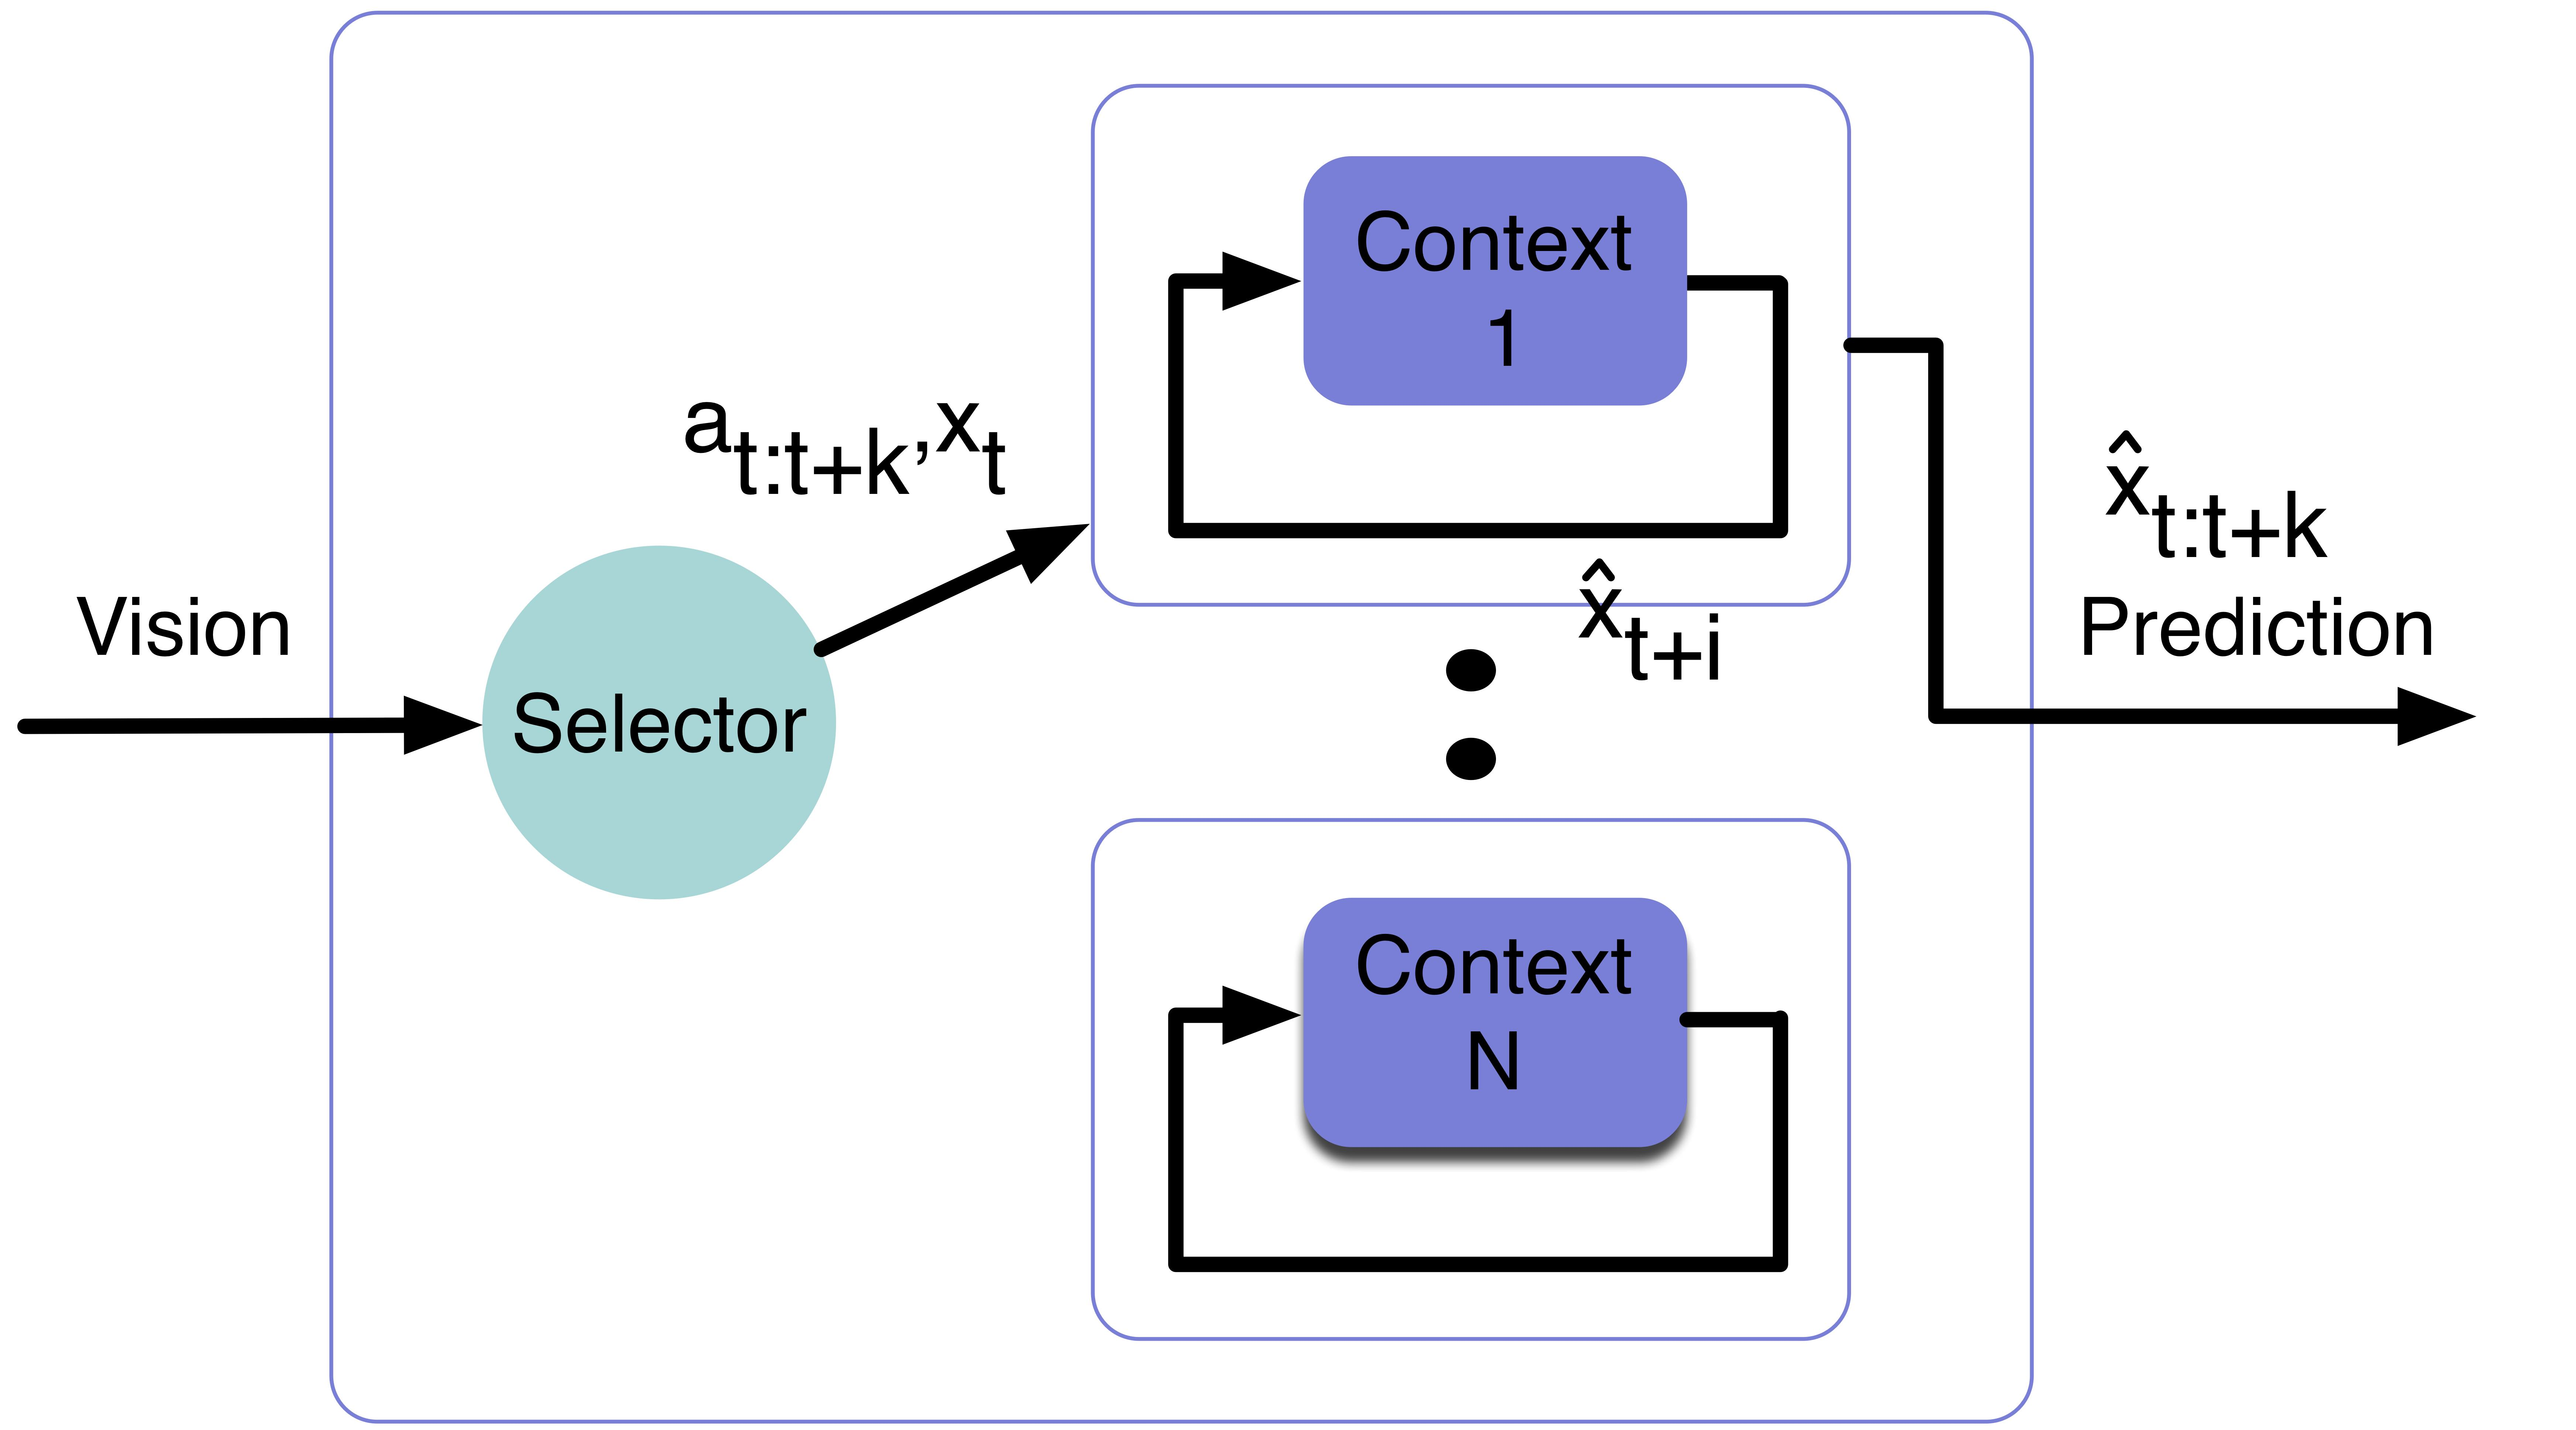
\includegraphics[width=0.9\columnwidth]{modular-schema}}
\caption{A modular prediction scheme for solving problem P1. Visual object identification selects a context/predictor, and gives it the object pose and intended finger trajectory as initial input. The chosen predictor takes the current system state $x_t$ and the planned manipulator trajectory $a_{t:t+k}$. The first prediction $\hat{x}_{t+1}$ is fed back on itself to produce a multi-step prediction $\hat{x}_{t:t+k}$. \label{fig:modular-simple}}
\end{figure}
In this paper we pursue a learning approach to prediction. We could try to learn a single predictor, applicable to a wide range of objects and contexts. This is hard, however, because a great deal must be captured in a single learner. Instead, we employ a modular prediction scheme, inspired by MOSAIC \citep{Haruno_MOSAIC_2008} and other models \citep{demiris2003distributed}. Modular means that the overall prediction engine consists of many context specific predictors (Figure~\ref{fig:modular-simple}), where a context is an object, or an object-environment combination. The first advantage of this is that it can be easier to solve many simple learning problems than one complex learning problem. Second, unobservable parameters (frictional coefficients, mass, mass distribution) need not be modelled explicitly, but are instead captured implicitly by being associated with a particular context. Whereas MOSAIC couples control and prediction, but avoids real objects (working with simulated mass spring systems). Our work focuses on pure prediction, but for real objects. Our modular prediction scheme uses vision to distinguish the context, by identifying an object shape from a library. We also show how to decompose the prediction models into recombinable components, by factoring them. The models are factored by the mechanical contacts. This factoring allows transfer learning.\footnote{This factoring could also be referred to as modular, in the sense that the factors can be combined and replicated. To avoid confusion, however, we use module only to refer to a context specific predictor. We use factoring to refer to elements in the recombinable scheme.}
\begin{figure*}[t]
\centerline{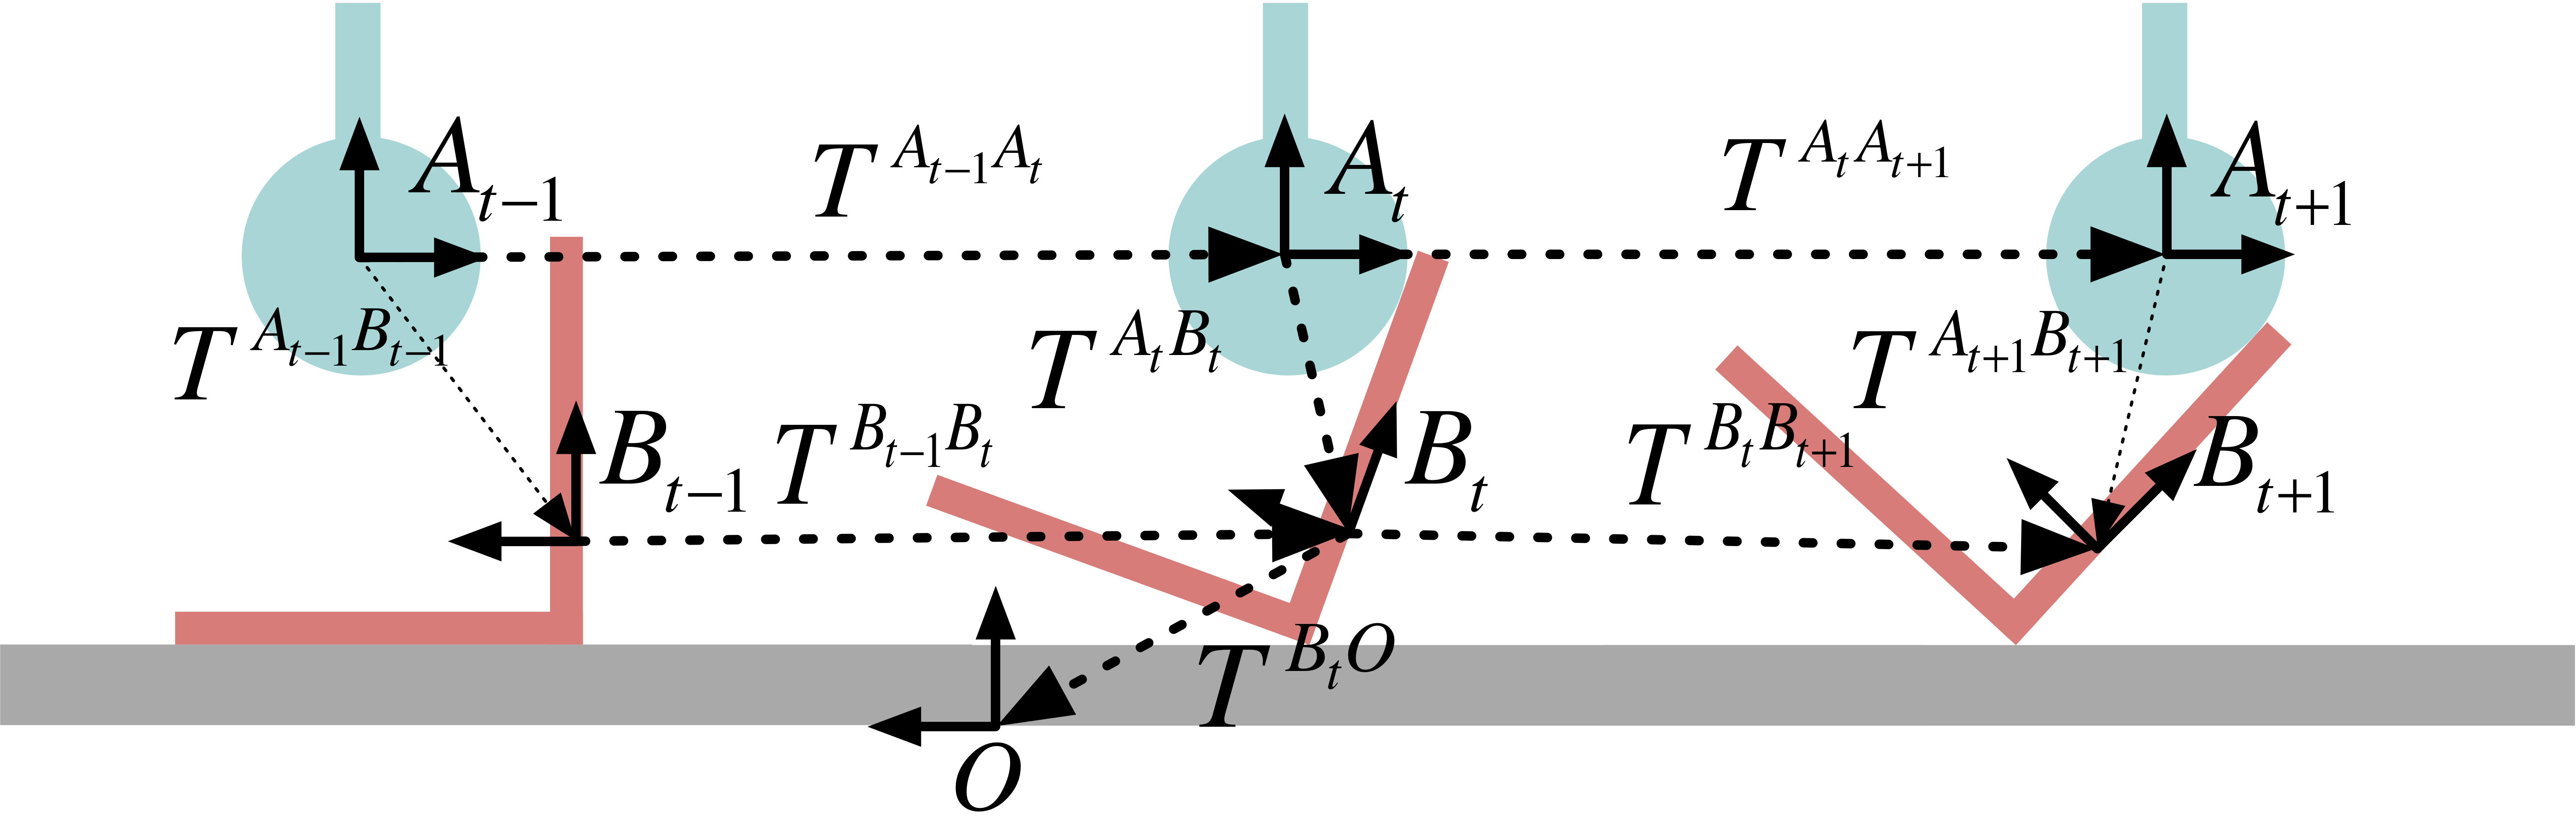
\includegraphics[width=0.8\textwidth]{sequential-frames}
%\includegraphics[width=0.34\textwidth]{similarity}
}
\caption[Setup1]{2D projection at time $t$ of a robotic finger with frame $A_{t}$ at time $t$,
an object with frame $B_{t}$, and a ground plane with constant frame
$O$. The system can be adequately described using six rigid body transformations. We show all the transformations referred to in the paper, marking the six transformations we use for framing our prediction problem as bold dotted lines, with the others shown as non-bold dotted lines. %$T^{A_t, B_t}$, $T^{B_t, O}$, $T^{A_{t-1}, A_{t}}$, $T^{A_{t}, A_{t+1}}$, $T^{B_{t-1}, B_{t}}$, and $T^{B_{t}, B_{t+1}}$.
}
\label{fig:Learning.setup1}
\end{figure*}
Having explained our overall scheme, we now turn to the mathematical details of how to model robot-object-environment interactions. This will lead, in turn, to posing the three prediction problems formally.